\documentclass[border=3pt, tikz]{standalone}

\usepackage{tikz}
\usepackage{amsmath}
\usepackage{nccmath}
\usepackage{pgfplots}

\pgfplotsset{compat=1.17}

\usepackage{xcolor}
\colorlet{myred}{red!80!black}
\colorlet{myblue}{blue!80!black}
\colorlet{mybluee}{myblue!80!black}
\colorlet{mygreen}{green!60!black}
\colorlet{myorange}{orange!70!red!60!black}
\colorlet{mydarkred}{red!30!black}
\colorlet{mydarkblue}{blue!40!black}
\colorlet{mydarkgreen}{green!30!black}

\begin{document}

\begin{figure}[!htbp]
  \resizebox{.75\textwidth}{!}{
    \begin{minipage}{0.35\textwidth}
      {\begin{center}
          \Large{\textbf{\textcolor{mygreen!60!black}{ELU}}}\end{center}}
      {\Large
        \begin{equation*}
          \textcolor{mygreen!60!black}{\begin{cases}
              \alpha \cdot \exp(z) - 1     \\
              z \qquad \text{if } z \geq 0
            \end{cases}}
        \end{equation*}
      }
    \end{minipage}
    \begin{minipage}{0.46\textwidth}
      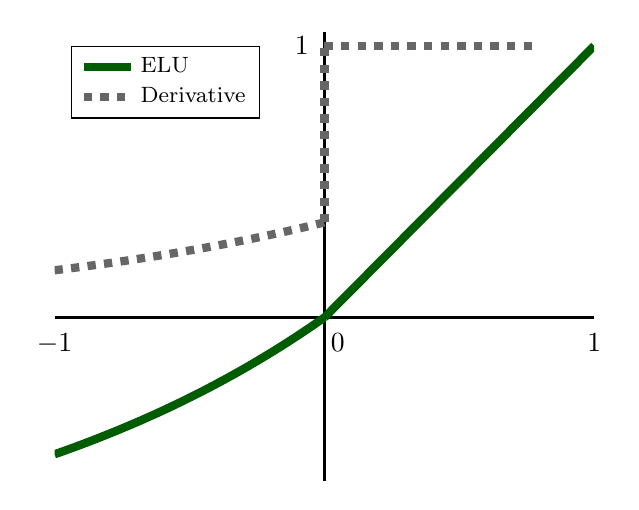
\begin{tikzpicture}
        \begin{axis}[
            axis lines=middle,
            xmax=2,
            xmin=-2,
            ymin=-0.6,
            ymax=1.05,
            xtick={-10, -2, 0.1, 2, 10},
            ytick={1},
            xticklabels={$-2$, $-1$, $0$, $1$, $2$},
            yticklabels={$1$},
            axis line style={-},
            axis line style ={very thick},
            tick style={draw=none},
            label style={font=\scriptsize},
            every axis x label/.style={at={(current axis.right of origin)},anchor=north west},
            every axis y label/.style={at={(current axis.above origin)},anchor=north east},
            legend pos=north west,
            legend style={font=\footnotesize},
            legend cell align={left},
          ]
          \addplot [line width=3pt, domain=-2:0, samples=100, mygreen!60!black]
          {exp(0.35*x)-1};
          \addplot [line width=3pt, domain=0:2, samples=100, mygreen!60!black,forget plot]
          {0.5*x};
          \addplot [line width=3pt, dashed, domain=-1:1, samples=100, gray!80!black]
          coordinates {(0,0.35) (0,1)};
          \addplot [line width=3pt, dashed, domain=-2:0, samples=100, gray!80!black]
          {0.35*exp(0.35*x)};
          \addplot [line width=3pt, dashed, domain=-1:1, samples=100, gray!80!black]
          coordinates {(0,1) (1.6,1)};
          \addlegendentry{ELU}
          \addlegendentry{Derivative}
        \end{axis}
      \end{tikzpicture}
    \end{minipage}
    \begin{minipage}{0.18\textwidth}
      \
    \end{minipage}
  }
\end{figure}

\end{document}